\documentclass[conference]{IEEEtran}
\IEEEoverridecommandlockouts
% The preceding line is only needed to identify funding in the first footnote. If that is unneeded, please comment it out.

\usepackage{cite}
\usepackage{amsmath,amssymb,amsfonts}
\usepackage{graphicx}
\usepackage{textcomp}
\usepackage{xcolor}
\usepackage{url}
\def\BibTeX{{\rm B\kern-.05em{\sc i\kern-.025em b}\kern-.08em
    T\kern-.1667em\lower.7ex\hbox{E}\kern-.125emX}}

\begin{document}

\title{Development of a Low-Cost Communication-Based Monitoring System Using Multiple Cameras for Wildlife Damage Control
%\thanks{Identify applicable funding agency here. If none, delete this.}
}

\author{\IEEEauthorblockN{Kota Sato}
\IEEEauthorblockA{\textit{Graduate School of Science and Technology} \\
\textit{Shinshu University}\\
Nagano, Japan \\
25w6039c@shinshu-u.ac.jp}
\and
\IEEEauthorblockN{Shungo Ito}
\IEEEauthorblockA{\textit{Graduate School of Science and Technology} \\
\textit{Shinshu University}\\
Nagano, Japan \\
25w6010e@shinshu-u.ac.jp}
\and
\IEEEauthorblockN{Shimpei Sato}
\IEEEauthorblockA{\textit{Faculty of Engineering} \\
\textit{Shinshu University}\\
Nagano, Japan \\
satos@shinshu-u.ac.jp}
\and
\IEEEauthorblockN{Daisuke Matsuo}
\IEEEauthorblockA{\textit{Organization for IT Initiatives} \\
\textit{Shinshu University}\\
Nagano, Japan \\
daisuke\_matsuo@shinshu-u.ac.jp}
\and
\IEEEauthorblockN{Lin Shan}
\IEEEauthorblockA{\textit{Organization for IT Initiatives} \\
\textit{Shinshu University}\\
Nagano, Japan \\
shanlin@shinshu-u.ac.jp}
}

\maketitle

\begin{abstract}
In recent years, agricultural damage caused by wildlife has become a serious issue, leading to an increased demand for trail camera systems that detect animal presence and immediately notify users.
However, conventional communication-based trail cameras face challenges such as high initial and running costs, as well as frequent empty shots caused by environmental factors like wind-blown vegetation.
These empty shots create a significant barrier due to the manual labor required to sort images visually.
To address these issues, this paper proposes a low-cost, communication-based monitoring system consisting of multiple low-cost edge cameras, an edge server, and a cloud server.
The edge server aggregates images from multiple cameras, reducing the number of required cellular contracts.
Furthermore, it filters images using YOLOv8n-based object detection and transmits only those highly likely to contain animals to the cloud, thereby reducing data traffic.
Field experiments showed that the proposed system reduced unnecessary image transmission by approximately 81.2\% during the daytime and 50.7\% at night.
Additionally, cost estimation based on a five-camera configuration showed that the system can reduce initial costs and operational costs compared to conventional LTE cameras.
\end{abstract}

\begin{IEEEkeywords}
Wildlife Damage Control, Trail Camera, YOLOv8, ESP32, Raspberry Pi
\end{IEEEkeywords}

\section{Introduction}
In recent years, agricultural damage caused by wildlife, such as sika deer and wild boars, has become a serious social problem in Japan. According to statistics from the Ministry of Agriculture, Forestry and Fisheries, the financial damage to crops caused by wildlife in FY2024 was approximately 18.8 billion yen, making wildlife damage control an urgent issue \cite{maff}.

To implement effective wildlife damage control measures, such as activating repellent devices in response to animal appearances or optimizing trap placement, it is crucial to grasp information on ``when'' and ``where'' target animals appear in real time. This is because real-time monitoring enables immediate countermeasures that cannot be achieved by post-data collection.

In conventional wildlife monitoring and damage control fields, automatic trail cameras equipped with Passive Infrared Ray (PIR) sensors have been primarily used. Conventional trail cameras do not have communication functions and generally record images on SD cards, which are collected and checked later. Recently, however, there have been attempts to automatically identify animal species using deep learning \cite{Tabak2019}, and systems that instantly notify users of captured images using LTE or satellite communication functions have been implemented \cite{Whytock2023,Patkar2025}. Furthermore, since the behavioral range of wildlife extends over vast agricultural lands and forests, it is essential to deploy many communication-based cameras and build a wide-area monitoring network to comprehensively grasp the appearance status in the target areas.

However, when deploying such existing communication-based trail cameras on a large scale, significant challenges arise in terms of cost and operational efficiency. First is the problem caused by empty shots. Because PIR sensors detect the movement of heat sources, they also react to wind-blown vegetation, resulting in many empty shots where no animals are captured. Consequently, users are required to manually sort images containing target animals from a vast amount of captured images, demanding significant labor. Second is the problem of initial and operational costs. When using cameras with LTE communication functions for real-time notification, not only are the cameras themselves expensive, but a communication contract is also required for each camera. Therefore, building a wide-area monitoring network incurs high initial and operational costs, which can be a barrier to adoption for general farmers and local governments.

In this study, we propose a low-cost, communication-based monitoring system consisting of inexpensive edge cameras, an edge server, and a cloud server. This system builds a closed local area network (WLAN) between multiple edge cameras and a single edge server in field environments without wired internet connections. By aggregating communications at the edge server, the operational costs associated with individual camera communication contracts are reduced. Furthermore, we adopt a two-stage processing architecture: preliminary filtering (hereafter referred to as primary selection) is performed using lightweight AI on the edge side to extract only images likely containing animals, and a large-scale AI on the cloud side makes the highly accurate final judgment regarding animal presence (hereafter referred to as re-evaluation). By dividing the judgment into two stages, we achieve a role division where the edge side discards empty shots to suppress communication traffic, while the cloud side prevents false alarms. This allows for the construction of a wide-area monitoring network with reduced initial and operational costs.

The structure of this paper is as follows. Section II describes related work. Section III explains the details of the proposed system. Section IV presents the experimental evaluation of the proposed system, and Section V discusses the experimental results. Finally, Section VI concludes this paper.

\section{Related Work}

The application of deep learning has been a widely noted approach in streamlining wildlife monitoring in recent years. Tabak et al. \cite{Tabak2019} trained Convolutional Neural Networks (CNN) models using a large-scale camera trap image dataset and demonstrated that automatic animal species identification was possible with an accuracy of over 98\%. MegaDetector \cite{Beery2019} is a pre-trained object detection model using camera trap images captured in various environments globally, capable of generically detecting animals, people, and vehicles. Fennell et al. \cite{Fennell2022} verified that MegaDetector has a high ability to minimize missed animals and can detect animals in images with high accuracy.

Regarding research emphasizing real-time performance, Whytock et al. \cite{Whytock2023} developed an instant alert system using satellite communication. However, the communication costs are extremely high, posing a significant barrier to widespread adoption by general farmers and local governments. As attempts to perform inference on edge devices, Patkar et al. \cite{Patkar2025} and Rahman et al. \cite{Computers2025} proposed high-performance monitoring systems using single-board computers like Raspberry Pi. Particularly in the study by Patkar et al., empty shot images are removed using YOLOv8n on the edge side, demonstrating that fast inference is possible even on inexpensive single-board computers like Raspberry Pi. However, these devices have relatively high power consumption, and long-term operation in mountainous areas without commercial power requires large batteries or solar panels, increasing equipment costs and installation difficulty.

As an approach to power saving, Sato et al. \cite{Sato2022} proposed a network architecture consisting of multiple child nodes and one parent node. This method showed the effect of reducing the operational cost and power consumption of the entire system by aggregating communication lines at the parent node. However, since their method performs animal detection using deep learning on the child nodes, a certain amount of computational resources and power is still required for each of the many deployed child nodes. Furthermore, Saito et al. \cite{IEICE2020} proposed a hierarchical control method combining a power-saving microcontroller and a high-performance single-board computer (Raspberry Pi), showing the possibility of building nodes that reduce standby power. Semba et al. \cite{SMC2024} developed an automatic tracking device using a PTZ camera and deep learning. However, these studies have been limited to verification in small-scale configurations, and wide-area communication network construction in actual field environments and practical filtering effects of empty shot images due to environmental noise have not been sufficiently verified.

\section{Proposed System}
As described in Section II, the widespread deployment of conventional monitoring systems in field environments faces challenges regarding the power consumption and computational resource constraints of edge devices, as well as the practical filtering of empty shot images. To overcome these challenges, this study applies the concept of line aggregation by Sato et al. \cite{Sato2022} and proposes a low-cost, communication-based monitoring system where functions are completely separated between extremely low-power edge cameras that only capture images and an edge server that handles inference and communication. The edge cameras do not perform inference processing; instead, they use low-power microcontrollers capable of long-term operation without solar panels, specializing only in image acquisition. By aggregating images from multiple cameras into one edge server, individual communication contracts for each camera are rendered unnecessary, significantly reducing the system's operational costs. Furthermore, we adopt a two-stage processing architecture: primary selection is performed using lightweight AI on the edge server to extract images potentially containing animals, and re-evaluation is performed with high accuracy using large-scale AI on the cloud server. This two-stage processing enables a role division where the edge side discards empty shots to reduce data traffic, while the cloud side's accurate judgment prevents false alarms during immediate notification. Through these approaches, we aim to overcome the power and resource constraints identified in related work and realize a system that simultaneously achieves ``real-time performance,'' ``reduction of empty shots,'' ``suppression of communication volume,'' and ``suppression of operational costs.''

This section describes the architecture and detailed processing flow of the proposed system.

\subsection{System Architecture}
The overall configuration of the proposed system is shown in Fig.~\ref{fig:system}. This system consists of the following three main nodes and the network connecting them:
\begin{enumerate}
    \item \textbf{Edge Camera}: Image acquisition and transfer to the edge server.
    \item \textbf{Edge Server}: Image aggregation, primary selection by lightweight AI, and transfer to the cloud server.
    \item \textbf{Cloud Server}: Re-evaluation by large-scale AI, data accumulation, and user notification.
    \item \textbf{Network Configuration}: Construction of communication paths between edges and the cloud.
\end{enumerate}

\begin{figure}[tb]
    \centerline{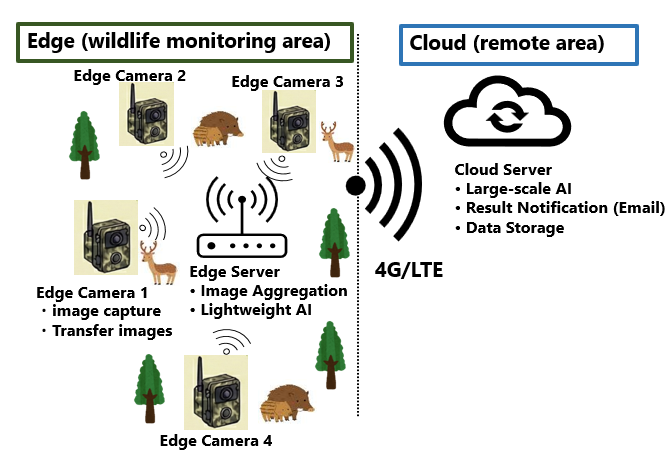
\includegraphics[width=\linewidth]{../img/system_structure_eng.png}}
    \caption{Overall architecture of the proposed system.}
    \label{fig:system}
\end{figure}

\subsubsection{Edge Camera}
Edge cameras are deployed directly throughout the monitoring area. They are responsible for detecting the appearance of animals, capturing images, and transferring them to the edge server via local communication. Since they are intended to be deployed in large numbers in outdoor environments without commercial power, they must use extremely low-power microcontrollers and be capable of operating for long periods solely on independent batteries.

In the implementation of this paper, we adopted the XIAO ESP32S3 Sense manufactured by Seeed Studio as the device. Although inexpensive, this device has Wi-Fi communication and camera functions. Furthermore, its Deep Sleep function minimizes power consumption during standby, aiming to fulfill the requirement for long-term operation. A PIR sensor is used as a trigger for motion detection, and HTTP communication via Wi-Fi is used to transmit images to the edge server. It uses eight AA batteries (6V) as a power source, facilitating installation in locations without power infrastructure. Fig.~\ref{fig:camera} shows an overview of the edge camera prototype.

\begin{figure}[tb]
    \centerline{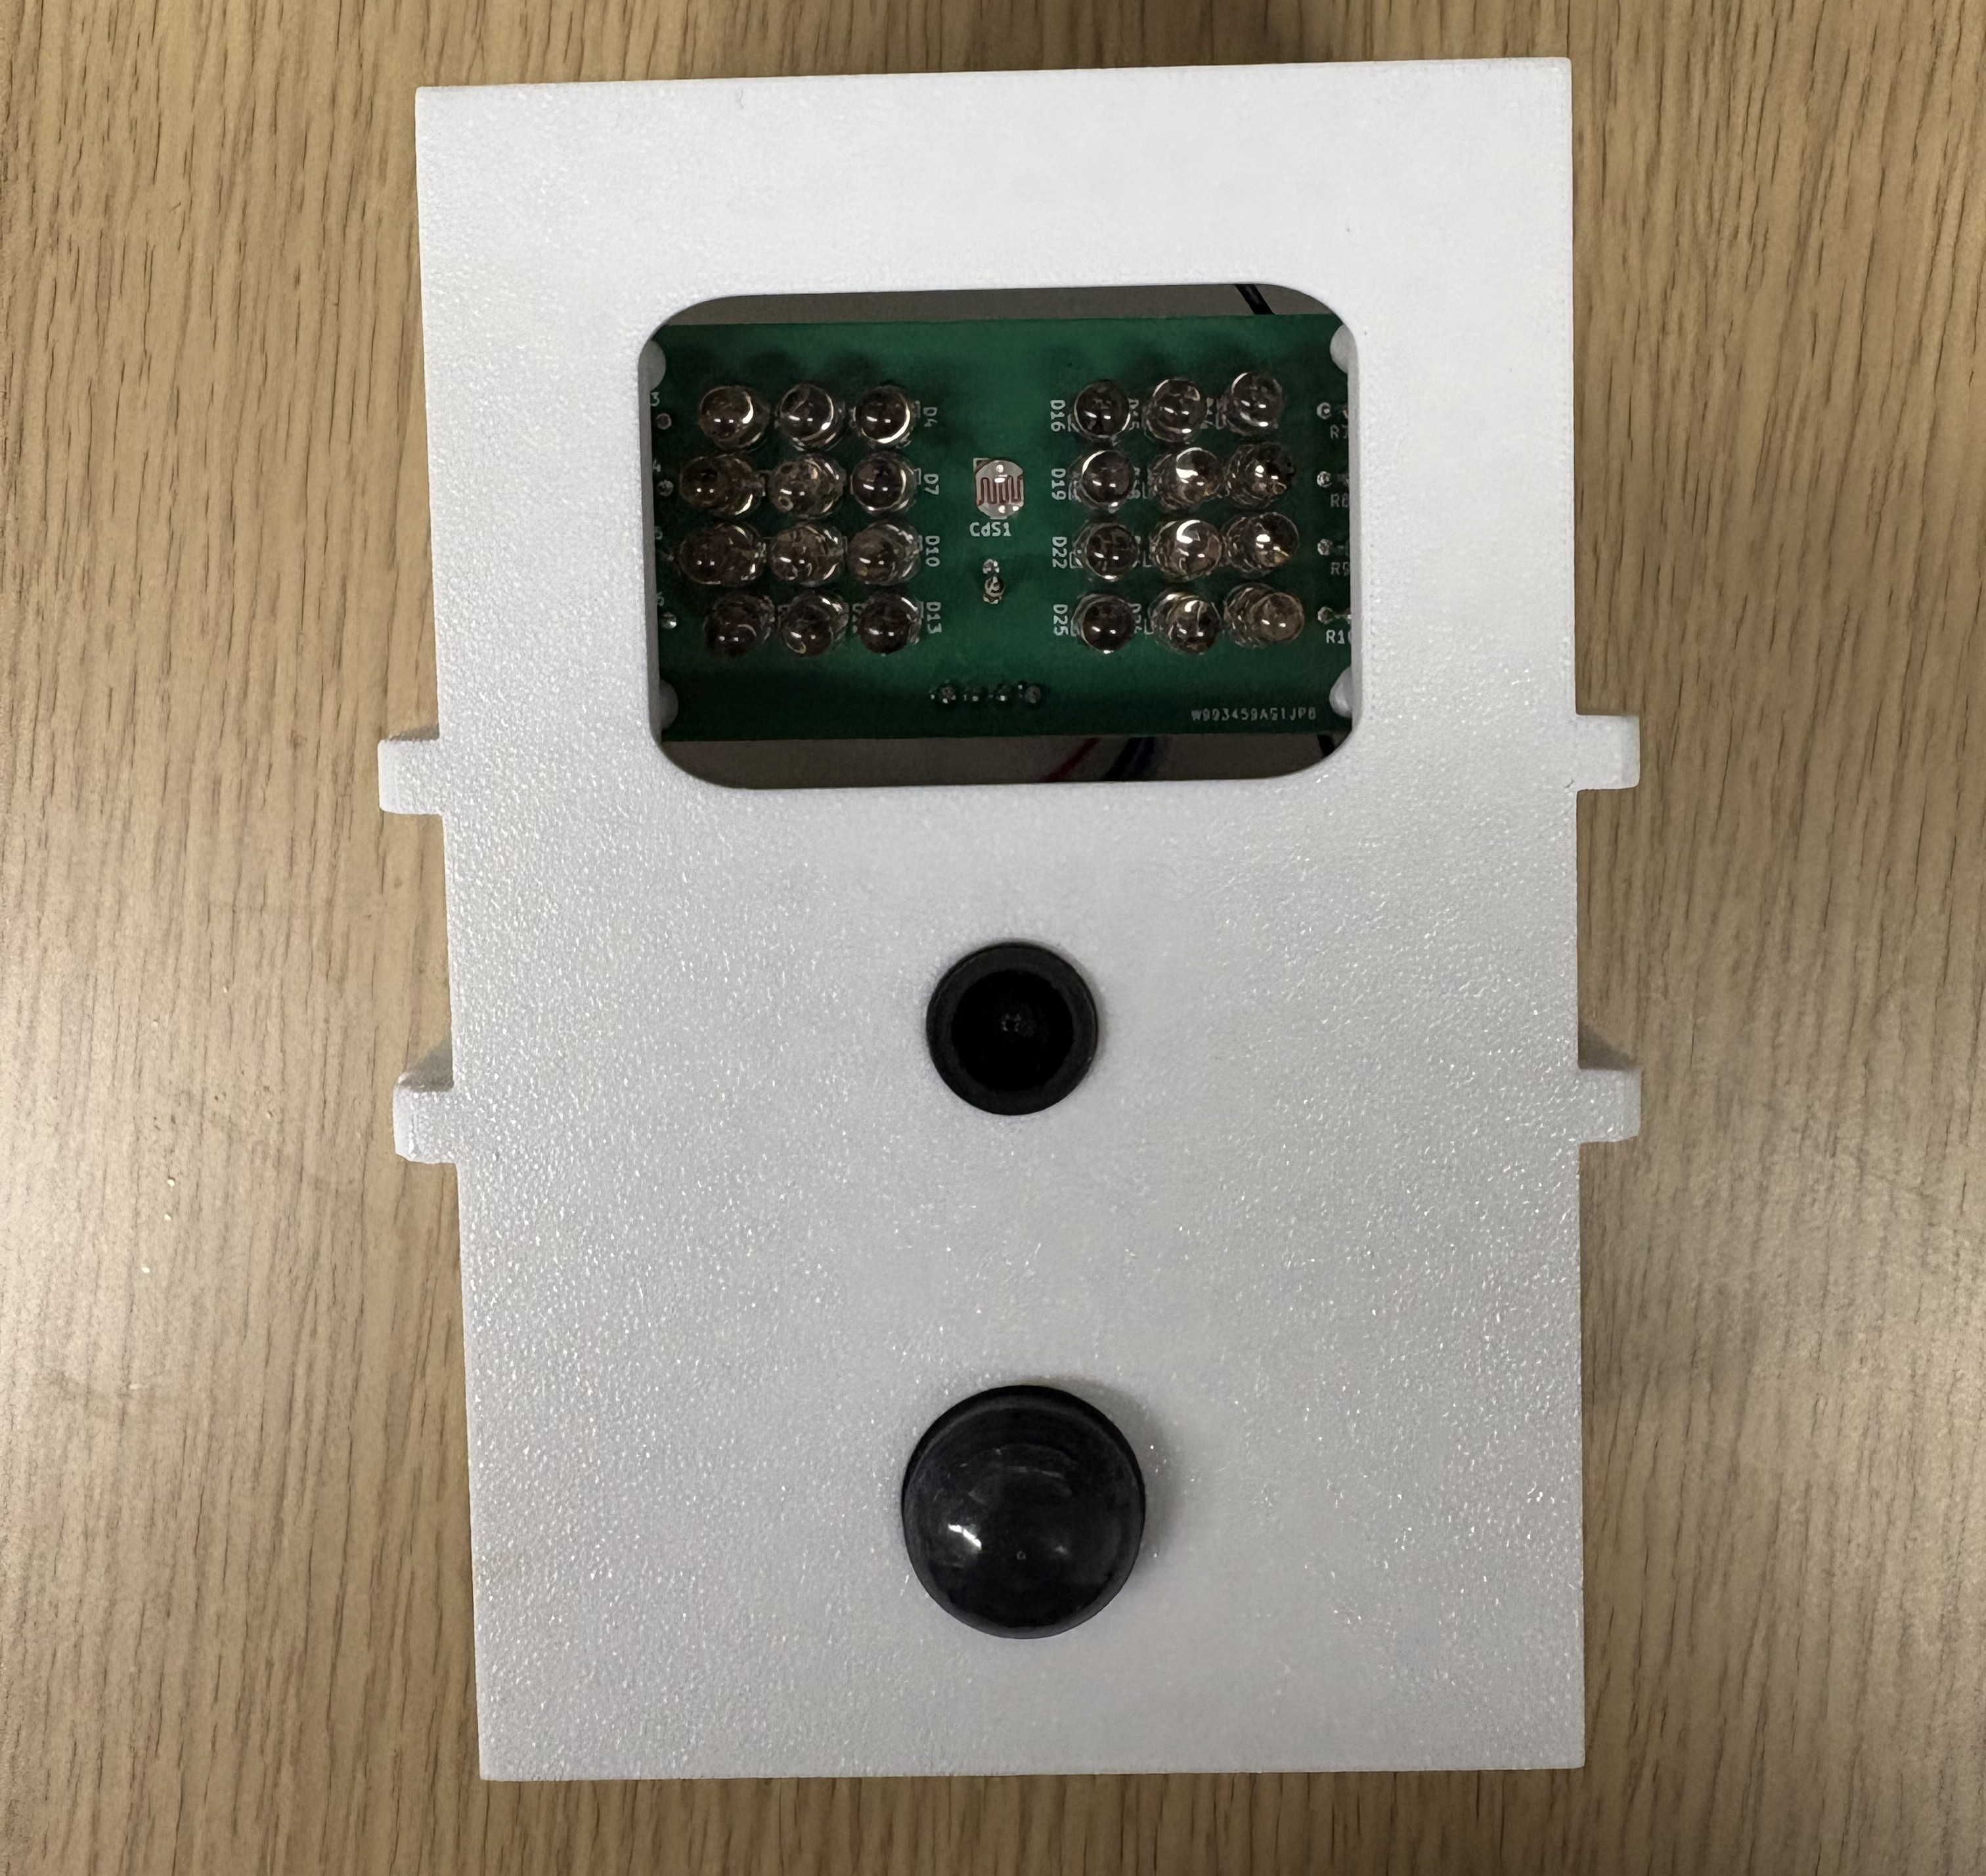
\includegraphics[width=0.6\linewidth]{../img/prototype_camera.jpeg}}
    \caption{Prototype of the edge camera.}
    \label{fig:camera}
\end{figure}

\subsubsection{Edge Server}
The edge server functions as a hub connecting multiple edge cameras and is responsible for reducing operational costs by aggregating communication lines. Simultaneously, it executes primary selection using lightweight AI at the edge to discard empty shot images and transfer only images containing animals, drastically reducing the communication volume to the cloud. To perform these processes autonomously in outdoor environments, the small computer and communication module must be capable of continuous operation using solar panels or similar power sources.

In our implementation, a Raspberry Pi 4B is used as the small computer, and an NEC Aterm HT100LN is used as the communication module. For the lightweight AI used for primary selection, we adopted YOLOv8n, pre-trained on the COCO dataset, which can perform inference at practical speeds even on devices with limited computational resources like the Raspberry Pi, while maintaining sufficient detection accuracy. HTTP communication is also used for transferring images to the cloud server. To operate this configuration continuously in an environment without commercial power, power equipment consisting of an approximately 200W solar panel and a 100Ah large-capacity battery is required based on estimates.

\subsubsection{Cloud Server}
The cloud server performs re-evaluation on images that passed the primary selection using a large-scale AI model, utilizing its abundant computational resources. This ensures accurate final determination of animal presence to prevent false alarms while immediately notifying the user when target animals are detected. In addition, it acts as a platform to centrally store received image data regardless of the judgment result, which can be utilized for future behavioral analysis or retraining AI models.

In our implementation, MegaDetector v5a is used as the large-scale AI model. MegaDetector is a pre-trained object detection model using images captured in diverse environments globally and possesses extremely high accuracy in animal detection, thus realizing reliable re-evaluation on the cloud server.

\subsubsection{Network Configuration}
Communication between devices in this system adopts a two-stage network configuration that considers operational costs and environmental constraints. The first stage is local communication between the edge cameras and the edge server. To prevent the increase in operational costs caused by contracting communication lines for each of the many edge cameras deployed in the monitoring area, a local network (WLAN) is built using a Wi-Fi access point installed on the edge server side. This aggregates images from multiple cameras to the edge server once, making individual communication contracts for cameras unnecessary. The second stage is wide-area communication from the edge server to the cloud server. Using an LTE communication module connected to the edge server, only images that passed the primary selection are transmitted to the cloud server via HTTP communication over the internet. This hierarchical network configuration realizes a mechanism to minimize communication costs while maintaining the scalability of the monitoring network.

In our implementation, the aforementioned NEC Aterm HT100LN is adopted as the core communication equipment to construct these networks. This device is connected to the edge server, utilizing its 2.4GHz Wi-Fi access point function to construct a local communication network with the edge cameras, while establishing a connection to the cloud using its LTE communication function.

\subsection{Data Processing Flow}
The data processing flow of the proposed system is shown in Fig.~\ref{fig:flow}. The layers cooperate to execute stages from image acquisition at the edge camera to primary selection at the edge server, and re-evaluation and notification at the cloud server. The processing flow of each component is described below.

\begin{figure*}[tb]
    \centerline{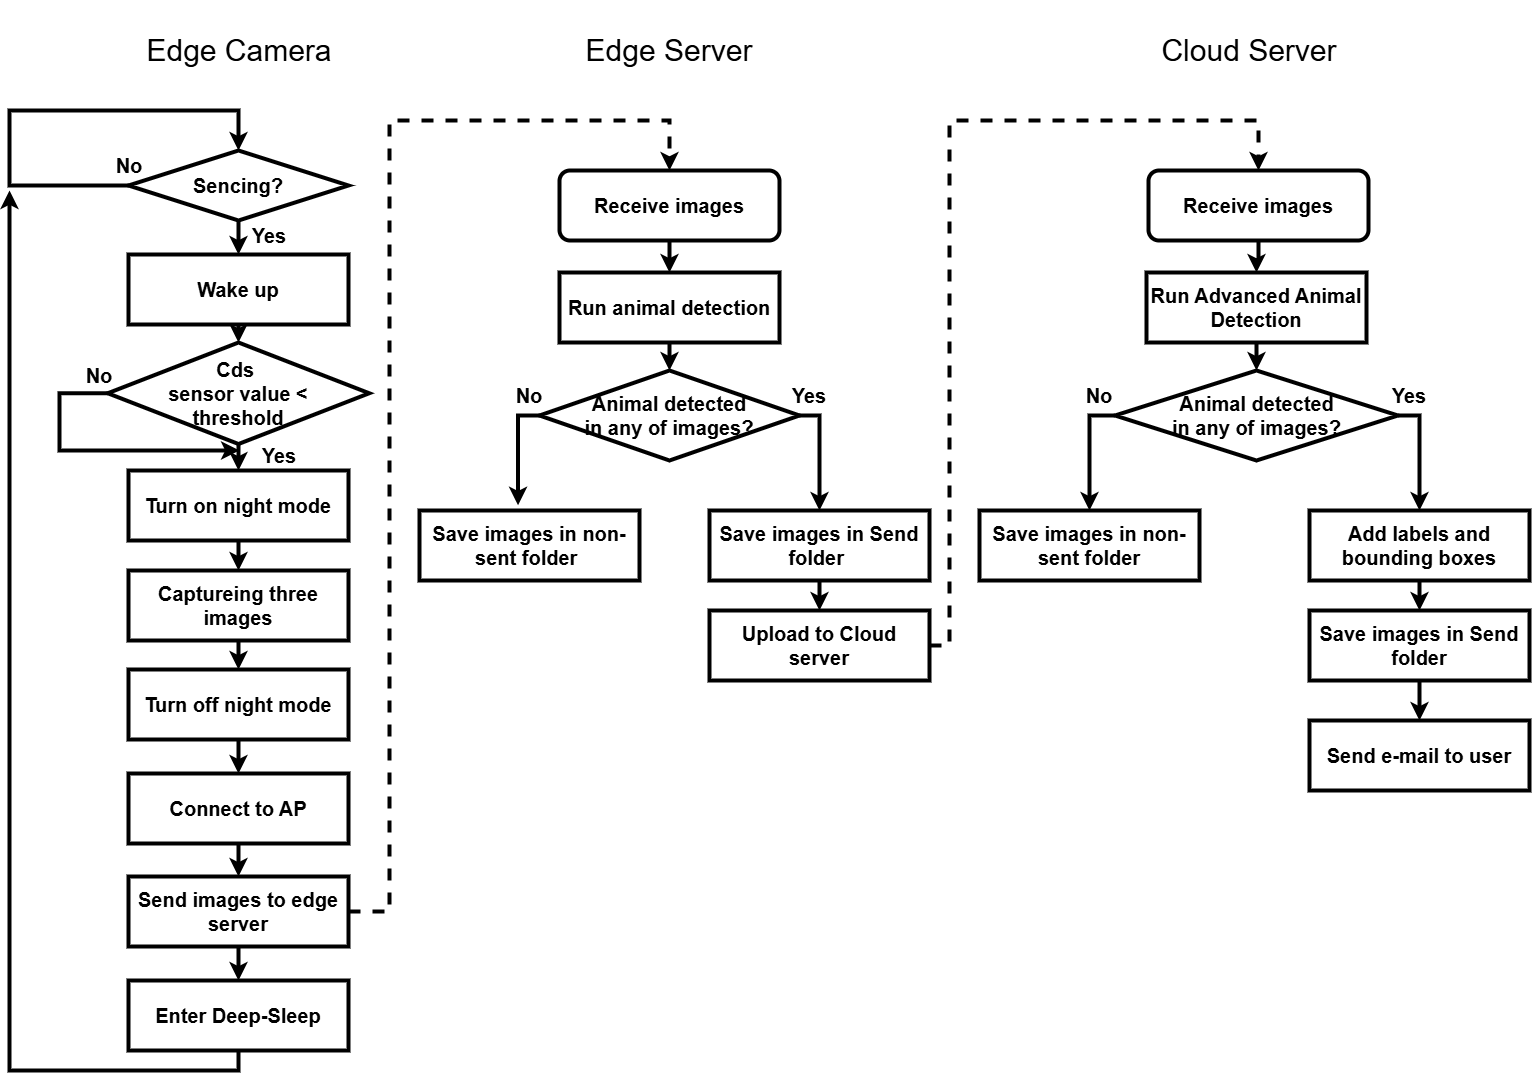
\includegraphics[width=0.85\linewidth]{../img/system_flow.png}}
    \caption{Data processing flow of the proposed system.}
    \label{fig:flow}
\end{figure*}

\subsubsection{Edge Camera Processing Flow}
The edge camera maintains a standby state using Deep Sleep mode and wakes up the moment the PIR sensor detects a heat source. After waking up, it captures three consecutive images in burst mode and immediately transmits them to the edge server via HTTP communication. After transmission is complete, the edge camera returns to the standby state after a certain interval, minimizing battery consumption.

\subsubsection{Edge Server Processing Flow}
The edge server constantly awaits image reception from edge cameras. Upon receiving images, it executes primary inference using YOLOv8n. If a class corresponding to an animal is detected in at least one of the three received images, the images are moved to a storage directory and transferred to the cloud server. If no animal is detected (e.g., empty shots due to swaying vegetation), the images are not transmitted, saving communication bandwidth.

\subsubsection{Cloud Server Processing Flow}
The cloud server constantly awaits transfers from the edge server. Upon receiving images, it re-detects animals using MegaDetector, a large-scale AI. Only when target animals are detected, it notifies the user of the appearance via email along with the image. Regardless of the judgment result, the images transferred from the edge server and the analysis results are accumulated in cloud storage. If no animal is detected, the system only accumulates the data and does not notify the user.

\section{Experimental Results with Prototype Implementation}
In this section, we describe the following four experiments conducted to verify the practicality of the proposed system:
\begin{enumerate}
    \item Measurement of power consumption during operation of each node.
    \item Evaluation of communication performance in an outdoor line-of-sight environment.
    \item Verification of object detection accuracy using a dataset collected in Kiso Town, Nagano Prefecture.
    \item Measurement of system processing time.
\end{enumerate}

\subsection{Experimental Environment and Parameters}
The equipment configuration used for the experiments is shown in Table \ref{tab:components}. Communication tests between the edge camera and the edge server were conducted in a line-of-sight outdoor environment on a sunny day.

\begin{table}[tb]
    \caption{System Components}
    \label{tab:components}
    \begin{center}
    \begin{tabular}{|l|l|l|}
        \hline
        \textbf{Component} & \textbf{Model} & \textbf{Specifications} \\
        \hline \hline
        \multicolumn{3}{|l|}{\textbf{Edge Camera}} \\
        \hline
        Main Unit & XIAO ESP32S3 Sense & 8MB PSRAM, 2.4GHz Wi-Fi \\
        \hline
        Camera Module & OV5640 & 2592$\times$1944 \\
        \hline
        PIR Sensor & Panasonic PaPIRs & Detection range $\sim$14m \\
        \hline
        Power Supply & 8 $\times$ AA batteries & 6V \\
        \hline \hline
        \multicolumn{3}{|l|}{\textbf{Edge Server}} \\
        \hline
        Main Unit & Raspberry Pi 4B & 4GB RAM \\
        \hline
        Power Supply & Recommended (Est.) & $\sim$200W panel, 100Ah battery \\
        \hline
        Comms Module & NEC Aterm HT100LN & LTE router \\
        \hline
    \end{tabular}
    \end{center}
\end{table}

\subsection{Power Consumption Evaluation of Edge Camera}
Because this system assumes operation in agricultural and mountainous areas where commercial power is difficult to access, the power consumption of each node is a critical indicator determining practicality. We measured the power consumption of the edge camera in each operating state (Table \ref{tab:camera_power}). At a power supply voltage of 5.0V, the current during standby was 114mA, and the maximum peak current during startup was 946mA.

\begin{table}[tb]
    \caption{Power Consumption of Edge Camera (5.0V)}
    \label{tab:camera_power}
    \begin{center}
    \begin{tabular}{|l|r|r|}
        \hline
        \textbf{Operating State} & \textbf{Current (mA)} & \textbf{Power (W)} \\
        \hline \hline
        Standby & 114 & 0.57 \\
        \hline
        Startup (Peak) & 946 & 4.73 \\
        \hline
        Wi-Fi Transmission & 250 & 1.25 \\
        \hline
    \end{tabular}
    \end{center}
\end{table}

\subsection{Power Consumption Evaluation of Edge Server}
We similarly measured the power consumption of the edge server (Raspberry Pi 4B). At a power supply voltage of 5.0V, the current consumption in the stable state (idle state) after system startup fluctuated between 405$\sim$410mA, and the average power consumption was about 2.05W. Adding the maximum power consumption of the LTE router (approx. 6W), the total power consumption of the edge server is approximately 8W.

\subsection{Communication Performance Between Edge Camera and Server}
Under a line-of-sight environment, we evaluated communication stability while varying the distance between the edge camera and the server. Table \ref{tab:comm_perf} shows the experimental results. At close range (approx. 1m), RSSI remained stable at around -30$\sim$-35dBm. At a distance of 100m, RSSI was around -60$\sim$-65dBm, and it dropped to -77$\sim$-80dBm at the maximum distance of 200m. While connection establishment and image transfer were successfully completed without problems up to 100m, approaching the 200m point caused RSSI to fall below -75dBm, resulting in noticeable latency and communication instability. Thus, in this configuration, stable image transfer is achieved up to about 100m in a line-of-sight environment, while communication quality degrades near 200m, suggesting that repeaters or alternative communication methods are necessary for stable operation over longer distances.

\begin{table}[tb]
    \caption{Communication Performance (Line-of-Sight Environment)}
    \label{tab:comm_perf}
    \begin{center}
    \begin{tabular}{|c|c|}
        \hline
        \textbf{Distance (m)} & \textbf{RSSI (dBm)} \\
        \hline \hline
        $\approx$ 1 & -30 $\sim$ -35 \\
        \hline
        $\approx$ 100 & -60 $\sim$ -65 \\
        \hline
        $\approx$ 200 & -77 $\sim$ -80 \\
        \hline
    \end{tabular}
    \end{center}
\end{table}

\subsection{Communication Reduction Effect by Edge Server}
We evaluated the object detection accuracy using YOLOv8 on the edge server and the resulting communication reduction effect. For images acquired in Kiso Town from June to November 2025, judgments by MegaDetector v5a (the large-scale AI model) were used as reference labels to evaluate the judgments of YOLOv8n on the edge server (Table \ref{tab:ai_accuracy}). To minimize missed animals (unintended image discarding) during the primary selection, the judgment threshold for YOLOv8n was intentionally set low at 0.05. Because this evaluation uses MegaDetector outputs as reference labels rather than human annotations, the obtained accuracy indicates the degree of agreement with MegaDetector rather than absolute performance against ground-truth labels. Here, Precision indicates the proportion of images that actually contained animals among those the AI judged as "animal present," and Recall indicates the proportion of images correctly detected by the AI among those that actually contained animals. Ref(MD) in the table represents the reference labels by MegaDetector.

\begin{table}[tb]
    \caption{AI Detection Accuracy (Daytime and Nighttime, Threshold: 0.05)}
    \label{tab:ai_accuracy}
    \begin{center}
    \scalebox{0.85}{
    \begin{tabular}{|c|c|r|r|r|r|}
        \hline
        \multicolumn{2}{|c|}{\textbf{}} & \multicolumn{2}{c|}{\textbf{Daytime (YOLOv8n)}} & \multicolumn{2}{c|}{\textbf{Nighttime (YOLOv8n)}} \\
        \cline{3-6}
        \multicolumn{2}{|c|}{\textbf{}} & \makebox[1.2cm][c]{\textbf{Pos.}} & \makebox[1.2cm][c]{\textbf{Neg.}} & \makebox[1.2cm][c]{\textbf{Pos.}} & \makebox[1.2cm][c]{\textbf{Neg.}} \\
        \hline \hline
        \textbf{Ref} & \textbf{True} & \textbf{195} & 13 & \textbf{104} & 48 \\
        \cline{2-6}
        \textbf{(MD)} & \textbf{False} & 73 & \textbf{1,147} & 28 & \textbf{88} \\
        \hline \hline
        \multicolumn{2}{|c|}{\textbf{Precision}} & \multicolumn{2}{c|}{72.8\%} & \multicolumn{2}{c|}{78.8\%} \\
        \hline
        \multicolumn{2}{|c|}{\textbf{Recall}} & \multicolumn{2}{c|}{93.8\%} & \multicolumn{2}{c|}{68.4\%} \\
        \hline
    \end{tabular}
    }
    \end{center}
\end{table}

The AI object detection accuracy resulted in a recall of 93.8\% and precision of 72.8\% during the daytime. Conversely, at night, the recall was 68.4\% and the precision was 78.8\%, showing a tendency for recall to decrease compared to daytime.

Next, Table \ref{tab:comm_reduction} shows the communication reduction rate. The communication reduction rate represents the proportion of events where the server judged "transmission unnecessary (no animal)" out of the total number of triggers (the number of times the PIR sensor reacted). In this evaluation, the three images captured per PIR trigger are treated as one cycle.

\begin{equation}
    \text{Reduction} = \left( 1 - \frac{\text{Transmitted Triggers}}{\text{Total Triggers}} \right) \times 100 \label{eq:reduction}
\end{equation}

\begin{table}[tb]
    \caption{Communication Reduction Rate by Day/Night}
    \label{tab:comm_reduction}
    \begin{center}
    \begin{tabular}{|l|r|r|}
        \hline
        \textbf{Item} & \textbf{Nighttime} & \textbf{Daytime} \\
        \hline \hline
        Total Triggers & 268 & 1,428 \\
        \hline
        Transmitted Triggers & 132 & 268 \\
        \hline
        Reduction Rate (\%) & 50.7 & 81.2 \\
        \hline
    \end{tabular}
    \end{center}
\end{table}

As a result, the communication reduction rate was 81.2\% during the daytime and 50.7\% at night, confirming a tendency for the reduction rate to be lower at night than during the day.

\subsection{Total System Processing Time}
We measured the overall system processing time in a good communication environment with an RSSI of around -35dBm. The processing time on the edge side (from camera capture to completion of transmission processing at the edge server) was approximately 33 seconds (total of approx. 20 seconds for camera processing and approx. 13 seconds for edge server processing). The processing on the cloud side (from reception to completion of email notification) took about 11 seconds. As a result, the total time required from detecting an animal to completing an email notification to the user was approximately 44 seconds.

\section{Discussion}

\subsection{Communication Reduction Effect and Object Detection Accuracy}
In the experimental results (Table \ref{tab:comm_reduction}), a high communication reduction rate of about 81.2\% was achieved during the daytime. This is because, while empty shots frequently occur during the day due to temperature changes from sunlight or vegetation swaying in the wind, the image processing side successfully judged these as ``no animal (True Negative).'' At night, because there are fewer empty shots due to temperature drops, the reduction rate was around 50\%, but it still successfully reduced unnecessary data by half. Overall, it is quantitatively shown that introducing this system can significantly suppress communication traffic compared to simply transmitting all captured images.

However, the Recall at night was relatively low at 68.4\%. This is likely due to the limitations of the lightweight YOLOv8n model, as well as the image quality of night shots (infrared irradiation range and noise). Because preventing missed detections is also crucial in wildlife damage control, it is necessary to improve recall for night images through model retraining and image processing.

\subsection{Practicality and Cost of the System}
From the communication performance experimental results, stable communication was confirmed within a distance of 100m in a line-of-sight environment. This suggests that the system has sufficient area coverage capability for general agricultural land and open forest environments. Furthermore, the overall system delay is about 44 seconds, meeting a certain standard for the immediacy required in wildlife damage control.

Considering the cost aspects of system introduction, commercial LTE cameras for wildlife damage control generally cost around 20,000 to 80,000 yen per unit as a reference value. On the other hand, the breakdown of material costs for the proposed system is approximately 8,000 yen per edge camera, 14,000 yen for the edge server unit, 33,000 yen for the server power system, and 13,000 yen for the LTE router. Assuming a configuration where cameras are installed at five points to monitor a wide area, the total material cost for five cameras (40,000 yen) and one edge server set (60,000 yen) is approximately 100,000 yen. While it is not appropriate to directly compare the selling price of commercial products with the material costs of a custom-built system, the proposed system is constructed using inexpensive generic components, achieving cost reduction in terms of unit component prices. Additionally, while conventional devices require a communication contract for each camera, the proposed system can aggregate communication lines for multiple cameras into one, explicitly demonstrating an expected reduction in operational costs.

\subsection{Energy Sustainability and Operational Load}
As a result of verification with the prototype, it was found that achieving long-term operation of the edge cameras, as outlined as a requirement in Section III.A.1, is difficult with the current hardware configuration. The standby power of the edge camera is 0.57W (114mA), which does not allow for several months of long-term operation on eight AA batteries. This is due to the hardware design of the XIAO ESP32S3 Sense used in this paper, where the SD card module and other components continue to consume power even during standby, and the power supply to them cannot be cut off from the microcontroller side. Furthermore, the power consumption of the edge server, including the LTE router, is about 8W, requiring a large-capacity power facility to achieve continuous operation without commercial power. As estimated, an approximately 200W solar panel and a 100Ah battery are required, leading to increased equipment costs and installation space. From the above, towards practical application, hardware improvements such as adding a circuit to control power supply to the SD card and camera module are essential for the edge cameras. For the edge server, to achieve sustainable operation, it is necessary to consider the introduction of large power systems as mentioned above or power-saving measures through intermittent operation.

\section{Conclusion}
In this paper, we proposed a low-cost, communication-based monitoring system with a three-layer structure consisting of edge cameras, an edge server, and a cloud server, aiming to reduce image review workload and initial/operational costs in wildlife damage control. Experimental results confirmed a communication reduction rate of approximately 81.2\% during the daytime and 50.7\% at night due to primary selection by YOLOv8n on the edge server. We also organized the material costs for a system assuming a five-camera configuration, demonstrating that in addition to suppressing initial costs using inexpensive generic components, operational costs can be reduced by aggregating multiple cameras into the edge server, which reduces the number of communication contracts.

On the other hand, the recall for night images remained at 68.4\%, leaving room for improvement from the perspective of suppressing missed animals. It was also revealed that the high power consumption of the edge cameras and edge servers poses a challenge for long-term unattended operation in the current configuration.

In the future, we plan to improve the detection model for night images, implement power supply control for the camera modules, and review the intermittent operation and power supply configuration of the edge server to enhance long-term operability in real environments. Furthermore, we will consider introducing LPWA (Low Power Wide Area) communication to expand the monitoring area and ensure communication stability in environments with many obstacles. Additionally, we will proceed with functional expansions to improve the practicality and convenience of the system, such as improving reduction rate and recall through transfer learning of the edge AI model, implementing an animal species classification function on the cloud side, and building a web interface for users.

\section*{Acknowledgment}

This research and development work was supported by the Ministry of Internal Affairs and Communications (MIC), Japan, awarded through the FORWARD program under grant \#JPMI250420001 (Principal Investigator: Lin Shan). This research was also conducted under the commissioned research ``Study on the Construction and Operation of a Wildlife Damage Control Model Utilizing IoT Technology in Kiso Town'' from Kiso Town, Nagano Prefecture. We would like to express our gratitude to Mr. Toshiyuki Nakamura of Kaida Kogen, Kiso Town, for providing the experimental field to conduct this research.

\bibliographystyle{IEEEtran}
\bibliography{refs_english}

\end{document}
